\chapter{Analiza tematu wyszukiwania tekstu}  % Analiza tematu
% 

%\begin{itemize}
%\item Jaki problem chcę (muszę :-) rozwiązać?
%\item Dlaczego rozwiązanie problemu jest ważne?
%\item Jak inni rozwiązują ten problem?
%\item Jakie są zalety i wady tych rozwiązań?
%\end{itemize}

%Odwołania do literatury:
%książek \cite{bib:ksiazka},
%artykułów w czasopismach \cite{bib:artykul},
%materiałów konferencyjnych \cite{bib:konferencja}
%i stron www \cite{bib:internet}.
%
%Równania powinny być numerowane
%wzór
%\begin{align}
%    y = \frac{\partial x}{\partial t}
%\end{align}
%
%
%\begin{itemize}
%\item analiza tematu
%\item wprowadzenie do dziedziny (\english{state of the art}) – sformułowanie problemu, 
%\item poszerzone studia literaturowe, przegląd literatury tematu (należy wskazać źródła wszystkich informacji zawartych w pracy)
%\item opis znanych rozwiązań, algorytmów, osadzenie pracy w kontekście
%\item Tytuł rozdziału jest często zbliżony do tematu pracy. 
%\item Rozdział jest wysycony cytowaniami do literatury \cite{bib:artykul,bib:ksiazka,bib:konferencja}. 
%Cytowanie książki \cite{bib:ksiazka}, artykułu w czasopiśmie \cite{bib:artykul}, artykułu konferencyjnego \cite{bib:konferencja} lub strony internetowej \cite{bib:internet}.
%\end{itemize}

%\begin{Definition}\label{def:1}
%Definicja to zdanie (lub układ zdań) odpowiadające na pytanie o strukturze „co to jest a?”. Definicja normalna jest zdaniem złożonym z 2 członów: definiowanego (łac. definiendum) i definiującego (łac. definiens), połączonych spójnikiem definicyjnym („jest to”, „to tyle, co” itp.). 
%\end{Definition}
%
%\begin{Theorem}[Pitagorasa]\label{t:pitagoras}
%W dowolnym trójkącie prostokątnym suma kwadratów długości przyprostokątnych jest równa kwadratowi długości przeciwprostokątnej tego trójkąta. 
%\end{Theorem}
%
%\begin{Example}[generalizacja]\label{ex:generalizacja}
%Przykładem generalizacji jest para: zwierzę i pies. Pies jest zwierzęciem. Pies jest uszczegółowieniem pojęcia zwierzę. Zwierzę jest uogólnieniem pojęcia pies.
%\end{Example}
\section{Sformułowanie problemu}
Wyszukiwanie tekstu w systemach towarzyszy ludziom od początków istnienia maszyn,
choć pierwsze komputery nie posiadały ogromnych ilość pamięci, co nie powodowało
potrzeby istnienia algorytmów wyszukujących tekst. Procesor Intel 8008 
zaprezentowany w 1972 posiadał jedynie 14-bitową magistralę adresową, co 
pozwalało na 16 KB pamięci \cite{bib:internet:Intel8008}. Obecna ilość pamięci,
którą otrzymujemy w sieci za pośrednictwem chmury Google - 15 GB \cite{bib:internet:GoogleCloud},
nieporównywalnie przewyższa ilość pamięci wykorzystywaną w projektach z tamtych
czasów.

Zasadniczym problem naszej pracy jest wyszukiwanie zawartości tekstowej
ogromnej ilość plików w różnych formatach. Takie podejście może okazać się 
problematyczne \newline w przypadku plików dźwiękowych, filmowych czy zdjęć
wszelkiego rodzaju.

\section{Dostępne rozwiązania} %state of art

Podjęcie problemu wyszukiwania plików po nazwach oraz zawartości jest bardzo
złożonym i trudnym problemem w sferze programistycznej. Istnieje wiele rozwiązań
tego problemu, które istnieją od początku pracy z komputerem. Narzędzia takie
jak \textbf{find}, \textbf{grep} czy \textbf{fzf} \cite{bib:internet:Fzf} pozwalają na wyszukiwanie
zawartości, która nas interesuje, ale kompleksowość tych narzędzi nie jest 
przystosowana do tak trudnego problemu, jakim jest wyszukiwanie treści w plikach,
które są zarchiwizowane. Z taką samą niedogodnością spotykamy się w przypadku
plików pochodzących z pakietu Microsoft Office 365, jednak jeśli rozwiążemy 
zadanie otrzymywania zawartości z archiwów, będziemy w stanie otrzymać również 
zawartość z plików z rozszerzeniami .doc, .docx czy .pptx.

\subsection{Przykładowe narzędzia dostępne do wykorzystania}

Narzędzie \textbf{find} to znane i popularne narzędzie wśród osób zaznajomionych z
technologiami Linuxa. Już bardzo często wykorzystywany do znajdowania plików
w systemie, jednak nie nadaje się do znajdowania zawartości plików.

\begin{figure}[h]
  \centering
\begin{tcolorbox}[
    colback=white,
    colframe=black,
    boxrule=0.5pt,
    arc=0pt
]
  \begin{minted}{bash}
find /biblioteka -name '*.pdf'
find /biblioteka -path 'książki/*.docx' 
find /biblioteka -name '*.py' -not -path '*/site-packages/*'  
find /biblioteka -maxdepth 1 -size +500k -size -10M           
find /biblioteka -type f -empty -delete 
  \end{minted}
\end{tcolorbox}
\caption{Przykład użycia programu find}
\label{fig:cmd:findExamples}
\end{figure}

Jak pokazano na rysunku \ref{fig:cmd:findExamples} te przykładowe komendy find
pozwalają na wyszukanie zawartości folderu biblioteka, a kolejne argumenty 
pozwalają na doprecyzowanie określonych właściwości pliku. Argument \textbf{-name}
pozwala na wyszukanie wszystkich słów odpowiadających nazwie pliku, jednak nie
uwzględniają ścieżki. Argument \textbf{-path} pozwala na wyszukanie plików, 
które odpowiadają podanej ścieżce, a nie jedynie nazwie pliku.

Połączenie argumentów \textbf{-name} oraz argumentu \textbf{-not} z \textbf{-path}
umożliwi wyszukanie tych plików, z rozszerzeniem .py, które nie znajdują się w
folderze paczek dodatkowych (ang. \english{site-packages}). Kolejna komenda 
wyszuka wszystkie pliki znajdujące się tylko w folderze /biblioteka (\textbf{-maxdepth 1})
oraz weźmie pod uwagę wszystkie pliki większe niż 500 KB i mniejsze niż 10 MB.

Ostatnia komenda z rysunku \ref{fig:cmd:findExamples} daje możliwość usunięcia 
\textbf{-delete} plików (nie folderów) \textbf{-type f}, które są puste \textbf{-empty}.

Do przeszukiwania zawartości plików dobrze nadaje się narzędzie grep, które jest
dostępny w każdej dystrybucji Linuxa. Jego działanie jest dość podobne do find'a,
gdyż posiada on możliwość wyszukiwania treść w plikach tekstowych. Grep nie 
posiada też możliwość szukania zawartości archiwów, plików .pdf oraz nie wspiera
formatów książkowych takich jak .djvu.

\begin{figure}[h]
  \centering
\begin{tcolorbox}[
    colback=white,
    colframe=black,
    boxrule=0.5pt,
    arc=0pt
]
  \begin{minted}{bash}
grep "szukany-tekst" /biblioteka/plik1.txt 
grep -r "szukany-tekst" /biblioteka 
grep -i "szukany-tekst" /biblioteka/plik1.txt
grep -w "szukany-tekst" /biblioteka/plik1.txt
grep -C 2 "szukany-tekst" plik1.txt
cat /biblioteka/plik1.txt | grep -v "szukany-tekst" 
  \end{minted}
\end{tcolorbox}
\caption{Przykład użycia programu grep}
\label{fig:cmd:grepExamples}
\end{figure}

Na rysunku powyżej możemy zobaczyć przykładowe komendy programu grep 
\ref{fig:cmd:grepExamples}. Pierwsza komenda wyszukuje tekst podany jako 
pierwszy argument w plik1.txt. Kolejna komenda pozwala nam przeszukać wszystkie 
foldery znajdujące się w folderze /biblioteka rekursywnie \textbf{-r}, gdzie 
zawartość plików posiada "szukany-tekst". Trzecia komenda wyszuka wszystkie 
instancje "szukany-tekst" ignorując przy tym wielkość liter. W tym przypadku 
można wyszukać tekst posiadający treść "szUKaNY-tEKst". Dodając argument \textbf{-w}
wyświetla się wiersza, w którym znajdowało się dopasowanie. 

Przedostatnia komenda w \ref{fig:cmd:grepExamples} pozwala na sprawdzenie 
kontekstu, w którym znajduje się znalezione ciąg znaków. Jeżeli "szukany-tekst" 
znajduje się w linii 25, to program przedstawi nam linie 23-27 z wyszczególnioną
treścią, którą wyszukiwano. Ostatnia komenda przedstawia, że program można 
wykorzystać, przyjmując zawartość innego programu przy pomocy standardowego 
wejścia strumieniowego. Ta komenda zwróci nam wszystkie linie, w których 
"szukany-tekst" nie występuje.

Istnieje również ripgrep, który jest następcą wcześniej wymienionego
narzędzia. Jego wydajność przewyższa grepa nawet trzydziestokrotnie w niektórych
testach wydajnościowych w wymiarze czasu. Nie jest on niestety domyślnie 
instalowany na większości systemów linuxowych. 

\section{Odniesienia do literatury}

Istnieje wiele odniesień do wyszukiwania danych w literaturze. Praca Google 
\cite{bib:internet:htmlSearchGoogle} odnosi się do problemu wyszukiwania tekstu 
w dobie internetu i ilości danych, która jest przechowywana w chmurze. Wymagane
jest indeksowanie, które przyspiesza wyszukiwanie, ale wykonane nie poprawnie 
skutkuje słabymi wyszukiwaniami. Ilość danych wydobywana i dostarczana do
użytkowników stanowi duże wyzwanie oraz wymaga wykorzystania skomplikowanych 
algorytmów. 

Należy również mieć świadomość, że wyszukiwanie tekstu html posiada dodatkową 
złożoność związaną z linkami (ang. \english{anchor}). Linki mogą prowadzić do 
kolejnych stron lub plików, które należy przeszukać w celu wydobycia informacji.
Powoduje to, że proste wyszukiwanie wymaga adaptacji kodu, aby odnieść się do 
przypadków, o których wcześniej nie wiedziano.

%W plikach, które znajdują się na stronach mogą być na przykład archiwa, które
%mają różne wielkości oraz różne typy kompresji. Dodatkowo kompresja może być 
%bardziej agresywna lub nawet stratna.

Podczas konferencji TREC \cite{bib:konferencja:TRECDuplicates} jeden z zespołów 
napotkał problem, duplikacji danych. Chęć wydobycia danych w celu utworzenia
tekstów wymagało usunięcia duplikacji dokumentów oraz wyborze tej treści,
która posiada najwięcej wartości. Mogłoby to być tematem rozszerzenie pracy. 

\section{Opis poznanych rozwiązań}
\subsection{Algorytm brute force}

\begin{figure}[h]
  \centering
  \begin{lstlisting}
for i := 0; i<len(pattern); i++{
  for j := 0; j<len(substring); j++{
    // compare bytes
  }
}
  \end{lstlisting}
  \caption{Przykład algorytmu brute force}
  \label{fig:code:bruteForceComparison}
\end{figure}

Jest wiele algorytmów, które wyszukują tekst. Jednym z takich algorytmów jest 
algorytm typu brute-force. Polega sprawdzaniu każdego bajtu, jego implementacja
jest bardzo prosta i standardowa, a złożoność czasowe tego rozwiązania wynosi
$O(len(pattern) * len(substring))$, gdzie len(pattern) to długość bloku 
przeszukiwanego, a len(substring) to długość tekstu szukanego. Ten algorytm nie 
pozwala na wykonanie optymalizacji wykorzystywanej w kolejnych algorytmach, 
takich jak przesunięcie się do następnej instancji znaku powtórzonego. 
Przykładową implementację algorytmu można znaleźć na rysunku
\ref{fig:code:bruteForceComparison}.


\begin{figure}[h]
  \centering
  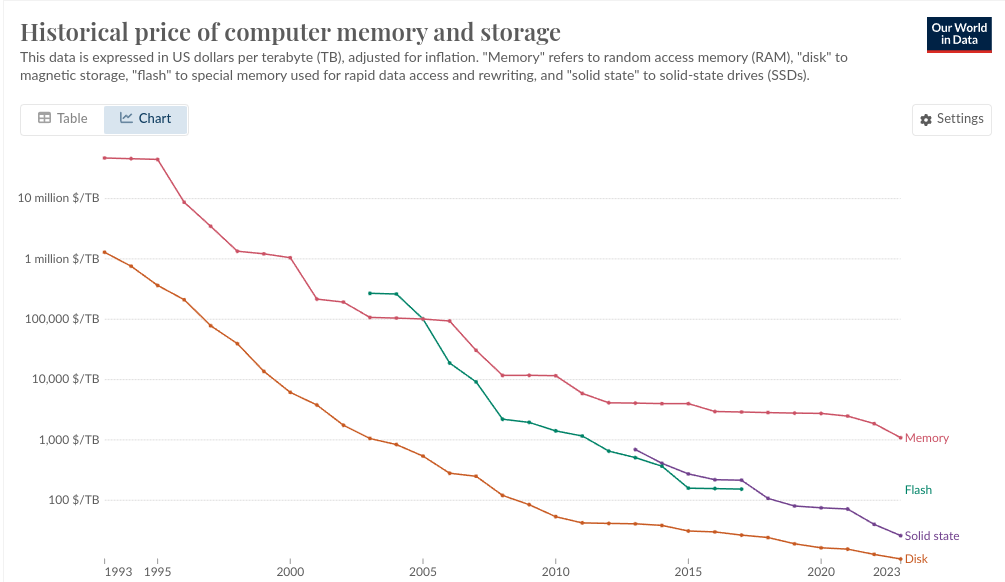
\includegraphics[width=0.9\textwidth]{./images/historical-mem-price.png}
  \caption{Historyczne dane cen pamięci w latach 1993-2023}
  \label{screenshot:MemPrices}
\end{figure}
%\cite{internet:HistoricalMemPrice}
%https://jcmit.net/memoryprice.htm

\subsection{Algorytm Morisa-Pratta}

\begin{figure}[h]
  \centering
  \begin{lstlisting}
preproc := make([]byte, len(substr)+1)
curr = -1
preproc[0] = -1
for i := 1; i <= len(substr); i++ {
  for (curr > -1) && (substr[curr] != substr[i-1]) {
    curr = preproc[curr]
  }
  curr++
  preproc[i] = curr
}
  \end{lstlisting}
  \caption{Przykład uprzedniego procesowania tekstu szukanego}
  \label{fig:code:preprocessMorisPratt}
\end{figure}

Algorytm Morisa-Pratta jest algorytmem, wykorzystującym możliwość procesowania 
łańcucha wyszukiwanego w tekście wykorzystując wcześniej pasującą do siebie część
(rys. \ref{fig:code:preprocessMorisPratt}).
Polega on na wykorzystaniu faktu istnienia pasującego prefikso-sufiksu.
Pozwala to na pominięcie porównania znaków, które się powtarzają w łańcuchu poszukiwanym.

Dzięki wykorzystaniu tej zależności możemy uniknąć cofania się indeksu i. 
Od teraz jako tablicę przechowującą informacje o przesunięciu w przypadku 
błędnego znaku, którą zainicjowaliśmy w \ref{fig:code:preprocessMorisPratt}
będziemy się odwoływać jako tablica \textbf{preproc}.
Tablice \textbf{preproc} wypełniamy poprzednią wartości tak długo, aż zaistnieje różnica 
pomiędzy obecnym a następnym znakiem tablicy poszukiwanej (tablicy \textbf{substr}). W przypadku różnicy 
zwiększamy wartość zapisywaną do tablicy \textbf{preproc} o odległość różnicy znaków.
W ten sposób następnym razem będzie możliwość pominięcia porównania tych znaków.

\begin{figure}[h]
  \centering
  \begin{lstlisting}
res := []int{}
curr := 0
found := 0
for i := 0; i < len(s); i++ {
  for (curr > -1) && (substr[curr] != s[i]) {
    curr = preproc[curr]
  }
  curr++
  if curr == len(substr) {
    for found < i-curr+1 {
      found++
    }
    res = append(res, found)
    found++
    curr = preproc[curr]
  }
}
  \end{lstlisting}
  \caption{Przykład procesowania łańcucha poszukiwanego w algorytmie Morisa Pratta}
  \label{fig:code:algoMorisPratt}
\end{figure}

W drugim etapie można wykorzystać wcześniej przygotowaną tablice przemieszczeń 
\textbf{preproc}, aby obliczyć ilość przesunięcia w przypadku znalezienia 
niepasującego prefiksu (rys. \ref{fig:code:algoMorisPratt}). Dzięki temu zwykle 
dłuższy tekst znajdujący się we wzorcu \textbf{s} możemy przeanalizować szybciej
niż w przypadku algorytmu brute-force. Powoduje to niestety problem w przypadku,
gdy wyszukiwany wzorzec nie jest wystarczająco długi, gdyż wykonanie operacji 
wcześniejszego procesowania posiada dodatkowy koszt, którego nie ma w algorytmie brute-force.

% \begin{minipage}[t][7cm][t]{\textwidth}
\vspace{-3cm} 
%   \centering
% \begin{minted}{go}
\begin{lstlisting}[basicstyle=\small]
func Index(s, substr string) int {
  n := len(substr)
	switch {
	case n == 0:
		return 0
  [...]
	case n > len(s):
		return -1
	case n <= bytealg.MaxLen: // Usually this case is used
		// Use brute force when s and substr both are small
		if len(s) <= bytealg.MaxBruteForce /* max == 64 */{
			return bytealg.IndexString(s, substr)
		}
  [...]
  }
}
\end{lstlisting}
\vspace{-.1cm} 
% \end{minted}
%   \caption{Szukanie łańcucha w standardowej bibliotece Golang}
%   \label{fig:code:golangSearchInsideString}
% \vspace{-1cm} 
% \end{minipage}

W podstawowej bibliotece języka Golang, w pakiecie \textit{strings} istnieje 
implementacja metody \textit{Index()}. Nie jest ona jednak w pełni przedstawiona
w kodzie, natomiast w jej implementacji można zauważyć, że algorytm brute-force
jest wykorzystywany tylko w przypadku, gdy długość wzorca wynosi więcej niż 64 
(rys. \ref{fig:code:golangSearchInsideString}). W Golang, gdy wzorzec jest większy niż
64 znaki, to wykonuje się algorytm podobny do Morisa-Pratta, który jednak 
posiada dodatkową walidację w przypadku odkrycia wyniku fałszywie dodatniego. 
Algorytm Morisa-Pratta nie potrzebuje takiej walidacji.

\subsection{Algorytm Kurta-Morisa-Pratta}

\begin{listing}[H]
    \begin{minted}[xleftmargin=0.15\textwidth,xrightmargin=0.2\textwidth,linenos]{diff}
preproc := make([]int, lensubstr+1)
preproc[0] = -1
curr := -1
for i := 1; i <= lensubstr; i++ {
  for (curr > -1) && (substr[curr] != substr[i-1]) {
    curr = preproc[curr]
  }
  curr++
- preproc[i] = curr
+ if (i == lensubstr) || (substr[i] != substr[curr]) {
+   preproc[i] = curr
+ } else {
+   preproc[i] = preproc[curr]
+ }
}
mp.preproc = preproc
    \end{minted}
  \caption{Różnica pomiędzy algorytmami KMP i MP}
  \label{fig:code:KurtMorisPrattVsMorisPratt}
\end{listing}

Kolejny rozpatrywany algorytm jest implementacja rozszerzająca poprzednią 
implementację przedstawioną w algorytmie Morisa-Pratta. Różnice można zauważyć na podstawie rysunku
(rys. \ref{fig:code:KurtMorisPrattVsMorisPratt}) i występuje w nim następująca różnica.
Gdy nie osiągnięto długości łańcucha i obecny znak jest równy temu, który 
znajduje się w łańcuchu szukany, to można wykonać skok do znaku znajdującego
się w tablicy przygotowanej, a nie sprawdzać kolejny znak w pętli. Ta różnica
powoduje, że algorytm wykonuje się szybciej.

Złożoność tego algorytmu wynosi $O(2*{len(pattern)})$, gdzie pattern to długość
tekstu przeszukiwanego. W najbardziej pesymistycznym przypadku, gdy próba dopasowania tekstu będzie 
kończyć się porażką, będzie to wymagało ilości operacji powrotu równej długości 
łańcucha szukanego. Powoduje to, że złożoność obliczeniowa sprowadza się do
$O({len(substr)}*{len(pattern)})$ co posiada tę samą złożoność co algorytm naiwny. 

\begin{table}
  \centering
  \begin{tabular}{ |c|c|  } 
    % \hline
    % \multicolumn{2}{|c|}{Przykład wykorzystania algorytmu KMP} \\
    \hline
    wzorzec S & AAAAAABAAAAAABAAAAAAA \\
    \hline
    łańcuch W & AAAAAA \\
    \hline
    liczba cofnięć & 20 \\
    \hline
  \end{tabular}
  \caption{Przykład wykorzystania algorytmu KMP}
  \label{tabela:KMPExampleSlow}
\end{table}

Wzorzec przeszukiwany T przedstawia najbardziej niekorzystny scenariusz 
(tab. \ref{tabela:KMPExampleSlow}), co można zaobserwować na przykładzie tekstu 
S = "AAAAAABAAAAAABAAAAAAA". W tym przypadku algorytm musi sprawdzić każde
wystąpienie 'A' przed dotarciem do 'B', co jest bardzo nieefektywne. Sytuacja 
pogarsza się wraz ze wzrostem liczby powtórzeń fragmentu "AAAAAAB". Mimo że 
metoda tablicowa działa tu sprawnie (bez potrzeby cofania się), to jej 
jednokrotne wykonanie dla łańcucha szukanego W może być wolny, gdyż proces
wyszukiwania często wymaga wielokrotnych przebiegów. Wielokrotne przeszukiwanie
tekstu S w poszukiwaniu wzorca prowadzi do gorszej wydajności. W takich 
przypadkach, gdzie mamy do czynienia z tego typu charakterystyką tekstu 
i wzorca, algorytm Boyera-Moore'a może stanowić optymalne rozwiązanie.

Algorytm KMP wykorzystuje w najgorszym przypadku liniowy przebieg, natomiast
algorytm Boyera-Moore'a w najlepszym przypadku posiada złożoność $O({len(wzorzec)}+{len(łańcuch)})$, a w 
najgorszym przypadku $O({len(wzorzec)}*{len(łańcuch)})$.

\subsection{Algorytm Boyera-Moore'a}
\label{sch:algoBoyerMoore}

Zaletą algorytmu jest to, że ilość skoków pomiędzy porównaniami jest zwykle 
większa od 1, a gdy istnieje sytuacja, w której litery w łańcuchu szukanym nie
powtarzają się, to możemy przeskoczyć o długość całego łańcucha szukanego.

Algorytm Boyera-Moore'a wprowadza rewolucyjne podejście poprzez skanowanie 
wzorca od prawej do lewej strony, w przeciwieństwie do MP i KMP, które 
analizują tekst od lewej do prawej. Ta fundamentalna różnica pozwala algorytmowi BM na 
znacznie efektywniejsze przeskakiwanie fragmentów tekstu, które na pewno nie 
zawierają wzorca. BM wykorzystuje dwie heurystyki: "złego znaku" oraz "dobrego
sufiksu", podczas gdy KMP i MP opierają się na pojedynczej tablicy prefiksowej.

W kontekście implementacji algorytm Boyera-Moore'a wymaga utworzenia dwóch tablic pomocniczych dla
swoich heurystyk, co zwiększa złożoność pamięciową w porównaniu do pojedynczej 
tablicy prefiksowej w KMP i MP. Jednak ta dodatkowa pamięć przekłada się na 
możliwość wykonywania większych skoków w tekście. KMP i MP różnią się między 
sobą głównie w sposobie konstrukcji tablicy prefiksowej. KMP wykorzystuje 
bardziej zaawansowaną technikę, która pozwala na uniknięcie niektórych 
niepotrzebnych porównań występujących w MP.

Praktyczny wybór między tymi algorytmami zależy od charakterystyki danych
wejściowych. BM sprawdza się najlepiej w przypadku długich wzorców i tekstów
napisanych w językach naturalnych, gdzie występuje duża różnorodność znaków.
KMP i MP są bardziej przewidywalne w działaniu i mogą być lepszym wyborem dla 
krótkich wzorców lub tekstów o ograniczonym alfabecie jak na przykład sekwencje
DNA.

Z tego też powodu należy wykonać heurystykę danych, które są analizowane.
Można to zrobić na kilka sposobów, jednak z powodu iż nie jest to główny temat
pracy, zostaną użyte narzędzia potrzebne do takiej analizy.


\subsection{TODO? Algorytm Karpa-Rabina}
\subsection{TODO? Algorytm Aho-Corasick}